\chapter{Routing Interior} \label{sec:int_routing}

\section{Configuração da Bancada e Tipologia de rede}

De forma a simular a tipologia de rede pretendida neste trabalho, as interfaces dos \textit{tuxs} foram configuradas da seguinte forma:

\begin{itemize}
    \item Tux 12 eth2 - 172.16.11.1/24
    \item Tux 13 eth1 - 172.16.11.2/24
    \item Tux 13 eth2 - 172.16.12.2/24
    \item Tux 14 eth1 - 172.16.12.3/24
\end{itemize}

\begin{figure}[H]
    \centering
    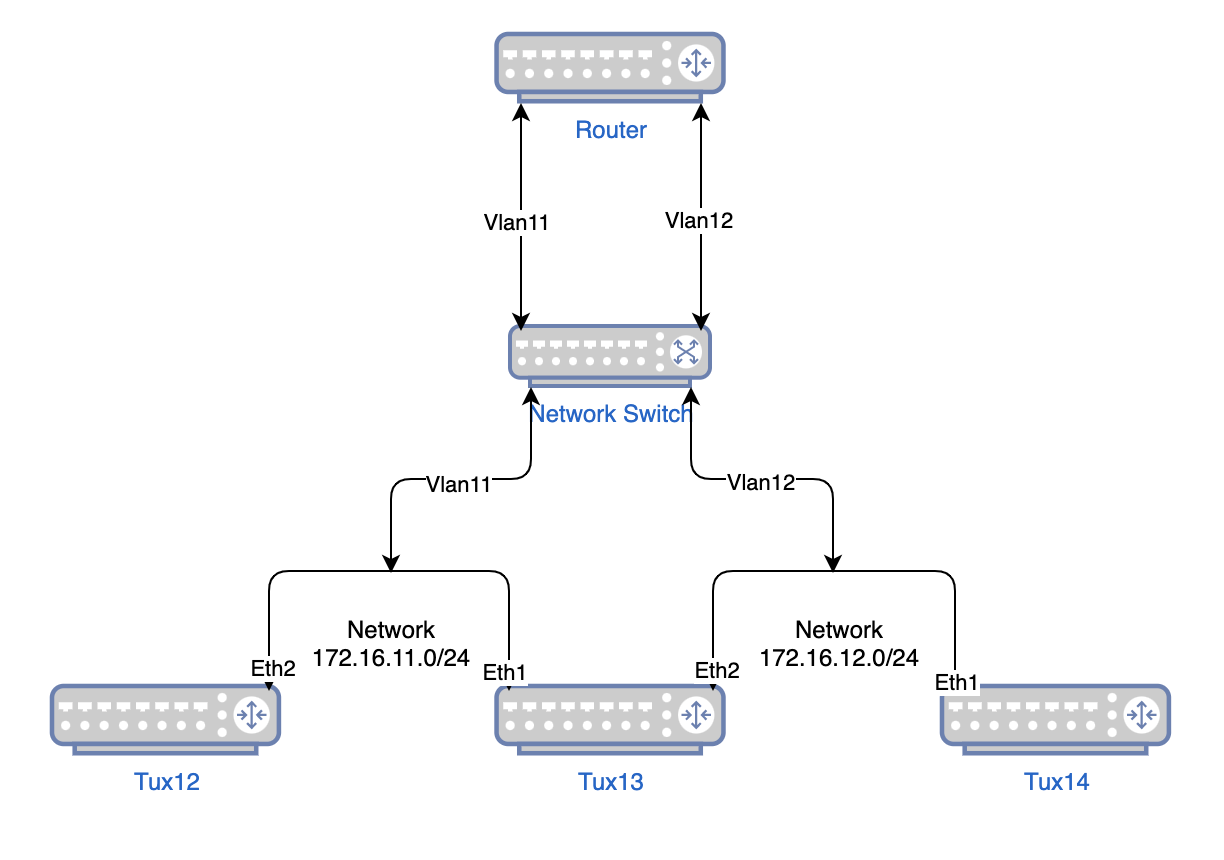
\includegraphics[width=.7\linewidth]{figs/int_routing/typo_net.png}
    \caption{Tipologia da rede}
    \label{fig:typo_net}
\end{figure}

Como observado na figura acima, é necessário criar duas Vlans separadas, de forma a simular duas \textit{networks} distintas.
Estas \textit{networks} estão ligadas entre si através de dois routers, o router de bancada, e o router no \textit{Tux13}.

\section{Configuração do Quagga}

O \textbf{Quagga} \cite{quagga} é um \textit{software} de routing que permite a implementação dos protocolos de \textit{routing}
\textbf{OSPF}, \textbf{BGP} e \textit{RIP}. Funciona sobre um \textit{daemon}, \textbf{zebra}, que cria uma \textit{layer} de abstração
ao \textit{kernel} do Linux, permitindo que diferentes serviços \textit{routing} operem entre os clientes do \textit{Quagga}.
Deste modo, este foi instalado em todos os \textit{tuxs}. 

O primeiro passo é especificar ao \textit{Quagga} quais os serviços ou \textit{daemons} que vão ser utilizados e que precisam de ser ativados.
Neste caso, o ficheiro \verb|/etc/quagga/daemons| foi configurado da seguinte forma:

\begin{center}
    \begin{itemize}
        \centering
        \item zebra = yes
        \item bgpd = no
        \item ospdf = yes
        \item ospf6d = no
        \item ripd = yes
        \item ripngd = no
    \end{itemize}
\end{center}

É também necessário ativar \textit{Packet Forwarding} IPv4.
Esta configuração está pro predefinição desativada dado que não se espera que um computador se comporte como um \textit{Router} em situações normais.
Isto é precisamente o que queremos que aconteça, sendo que esta funcionalidade foi ativada com o comando:

\begin{center}
    \centering
    \verb|echo 1 > /proc/sys/net/ipv4/ip_forward|
\end{center}

\section{Configuração do \textit{daemon} Zebra}

O Zebra, tal como indicado anteriormente, é o \textit{daemon} que permite correr os protocolos de routing sobre o \textit{kernel} do Linux.
Para configurar o Zebra, é preciso modificar o seu ficheiro .conf. Dado que por predefinição nenhum existe, copiamos o ficheiro \textit{default}
do diretório \verb|/usr/share/doc/quagga-core/examples/zebra.conf.sample| para o diretório do quagga \verb|/etc/quagga/zebra.conf|.

Neste ficheiro, especificamos vários componentes \cite{zebra}:
\begin{itemize}
    \item Host-name: O nome do Router que vai operar no computador
    \item Password: Password para acesso root ao terminal do Router
    \item Log file: Ficheiro onde se vai registar as operações do serviço
    \item Interfaces (e respetivos IPs) que vão ser usadas no routing
\end{itemize}

\begin{figure}[H]
    \centering
    \begin{subfigure}[b]{0.49\textwidth}
        \centering
        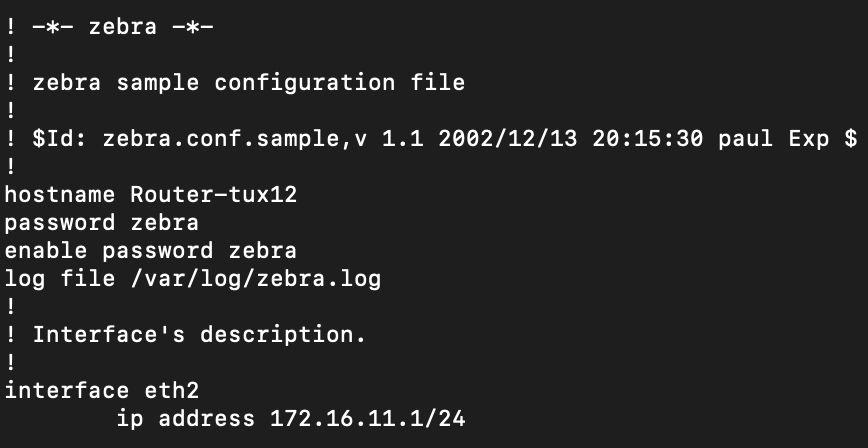
\includegraphics[width=.9\linewidth]{figs/int_routing/zebra_tux12.png}
        \caption{Ficheiro zebra.conf no Tux12}
        \label{fig:zebra_tux12}
    \end{subfigure}
    \begin{subfigure}[b]{0.49\textwidth}
        \centering
        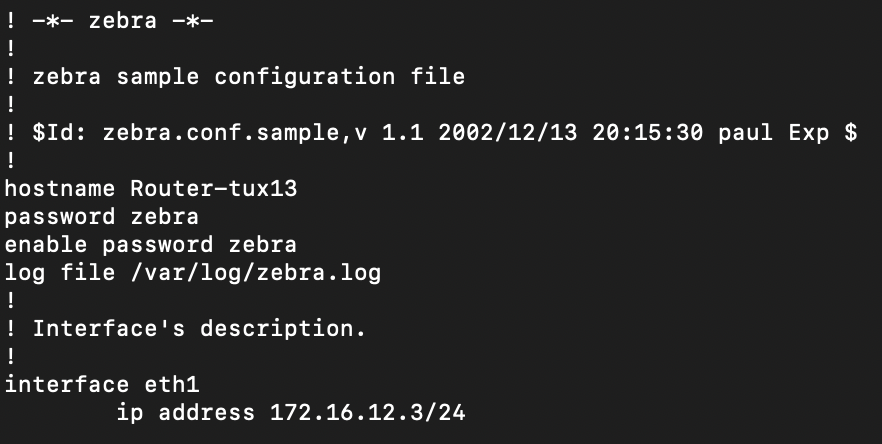
\includegraphics[width=.9\linewidth]{figs/int_routing/zebra_tux14.png}
        \caption{Ficheiro zebra.conf no Tux14}
        \label{fig:zebra_tux14}
    \end{subfigure}
\end{figure}

\begin{figure}[H]
    \centering
    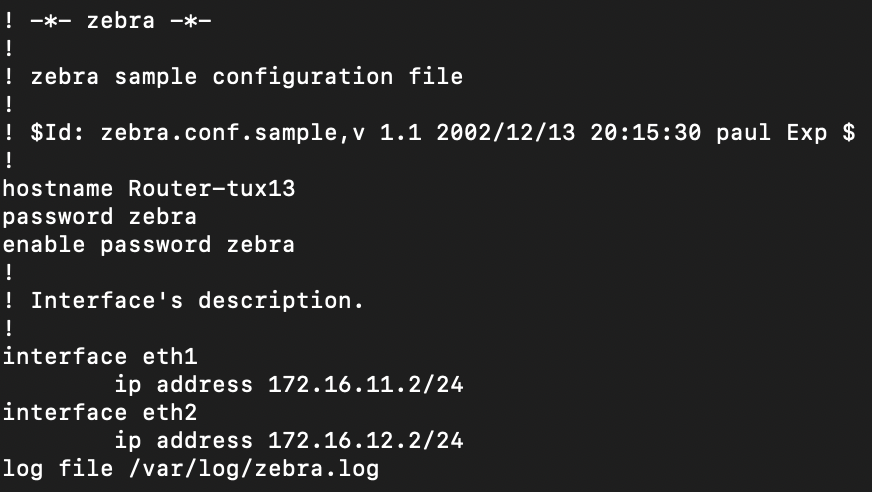
\includegraphics[width=.7\linewidth]{figs/int_routing/zebra_tux13.png}
    \caption{Ficheiro zebra.conf no Tux13}
    \label{fig:zebra_tux13}
\end{figure}

Neste ficheiros de configuração, especificamos as interfaces associadas ao serviço \textit{Zebra}, que neste caso apenas vai ter o sub-serviço \textit{OSPF}.
Atribuímos também os IPs associados a cada interface, eliminando a necessidade de os configurar manualmente.


O passo seguinte consiste na configuração do \textit{OSPF}.
O serviço é criado com o comando \verb|router ospf|, especificando-se a \textit{network} e \textit{area} onde opera.
Consequentemente, especificamos as interfaces usadas no serviço \textit{OSPF}.

\begin{figure}[H]
    \centering
    \begin{subfigure}[b]{0.49\textwidth}
        \centering
        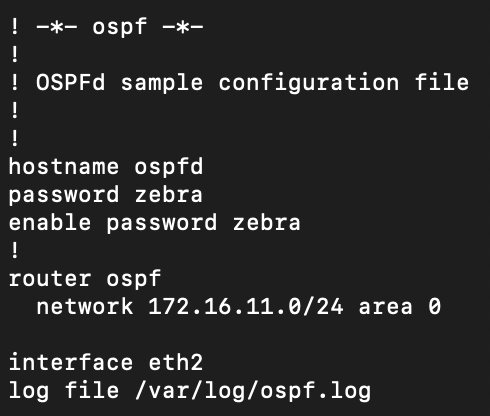
\includegraphics[width=.9\linewidth]{figs/int_routing/ospf_tux12.png}
        \caption{Ficheiro ospf.conf no Tux12}
        \label{fig:ospf_tux12}
    \end{subfigure}
    \begin{subfigure}[b]{0.49\textwidth}
        \centering
        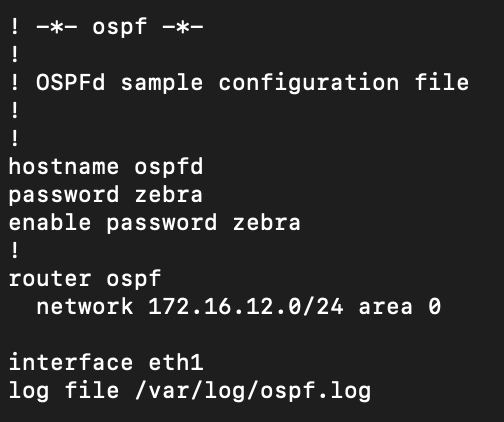
\includegraphics[width=.9\linewidth]{figs/int_routing/ospf_tux14.png}
        \caption{Ficheiro ospf.conf no Tux14}
        \label{fig:ospf_tux14}
    \end{subfigure}
\end{figure}

\begin{figure}[H]
    \centering
    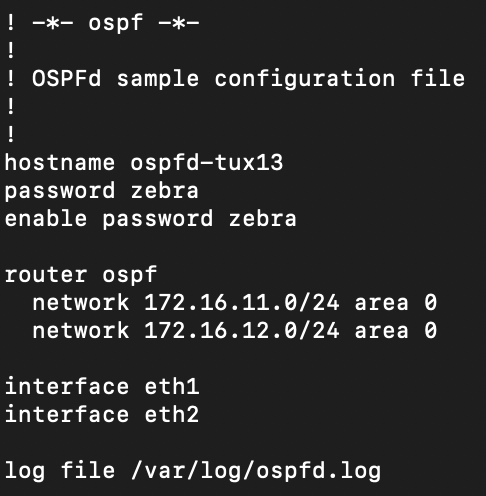
\includegraphics[width=.65\linewidth]{figs/int_routing/ospf_tux13.png}
    \caption{Ficheiro ospf.conf no Tux13}
    \label{fig:ospf_tux13}
\end{figure}

\pagebreak

\section{Configuração da Switch e Router}

O primeiro passo consiste em separar as duas \textit{networks} em \textit{Vlans} diferentes.

A \textbf{Vlan11} corresponde à rede \verb|172.16.11.0\24|.
Paralelamente, a \textbf{Vlan12} corresponde à rede \verb|172.16.12.0\24|.
Estas duas redes não estão conectadas entre si, pelo que a comunicação só pode ser feita numa layer superior,i.e., nos routers.

À rede \verb|172.16.11.0\24| pertencem as interfaces \textbf{Tux12-eth2} e \textbf{Tux13-eth1}.
À rede \verb|172.16.12.0/24| pertencem as interfaces \textbf{Tux13-eth2} e \textbf{Tux14-eth1}.


\begin{figure}[H]
    \centering
    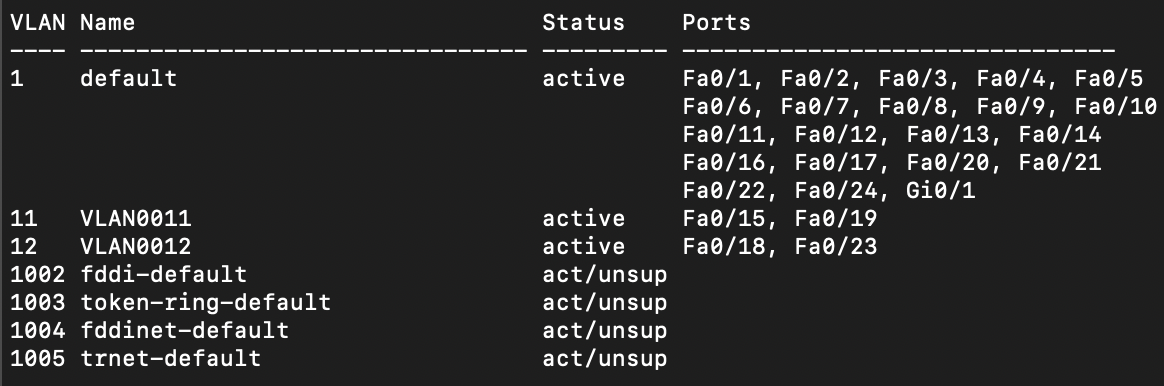
\includegraphics[width=.8\linewidth]{figs/int_routing/switch_1.png}
    \caption{Vlans no Switch}
    \label{fig:switch_1}
\end{figure}

\begin{figure}[H]
    \centering
    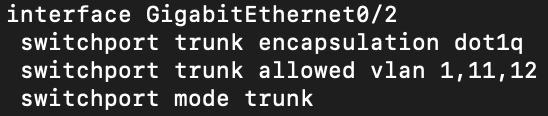
\includegraphics[width=.7\linewidth]{figs/int_routing/switch_2.png}
    \caption{Trunk para o Router}
    \label{fig:switch_2}
\end{figure}

No router de bancada, é feita a discriminação das duas Vlans em sub-interfaces diferentes de forma a separar o tráfego que chega.
Isto é feito através do encapsulamento configurado no Switch.

\begin{figure}[H]
    \centering
    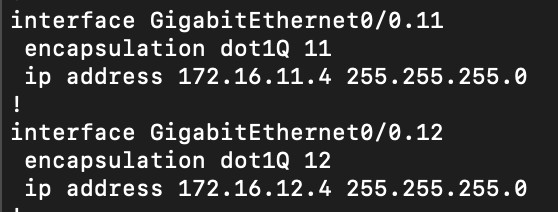
\includegraphics[width=.7\linewidth]{figs/int_routing/router_1.png}
    \caption{Interfaces no Router de Bancada}
    \label{fig:router_1}
\end{figure}

\section{Configuração do OSPF no Router}

Com o serviço OSPF configurado no 3 \textit{Tuxs}, também é preciso configurar o OSPF no próprio router \cite{cisco_ospf}.

\begin{figure}[H]
    \centering
    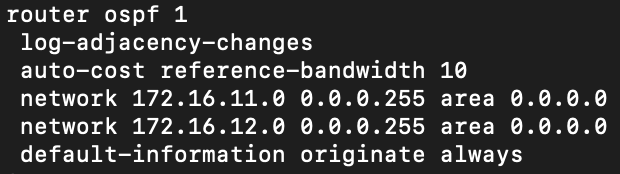
\includegraphics[width=.9\linewidth]{figs/int_routing/router_ospf.png}
    \caption{COnfiguração do OSPF no Router de Bancada}
    \label{fig:router_ospf}
\end{figure}

Nesta configuração, especificamos as duas \textit{networks}, correspondentes às diferentes \textit{Vlans}.
O comando \verb|default-information originate| especifica aquele router como a a rota \textit{default} para comunicações.

O comando \verb|auto-cost reference-bandwidth ref-bw| aplica um custo similar para as interfaces do router.
Isto deve-se ao facto das interfaces que ligam ao Router serem \textit{GigaBit}, enquanto que as que entre os Tuxs (no Switch) são \textit{Fast Ethernet}.
Isto resulta em custos diferentes para as rotas. De forma a uniformizar todos os custos, este comando foi executado quer no Router, quer nos serviços OSPF dos \textit{Tuxs} para garantir custo uniforme de 1.

\pagebreak

\section{Teste de conectividade}

Para garantir a conectividade entre todos os sistemas, efetuamos os normais testes \textit{ping} para todas as interfaces.

\begin{figure}[H]
    \centering
    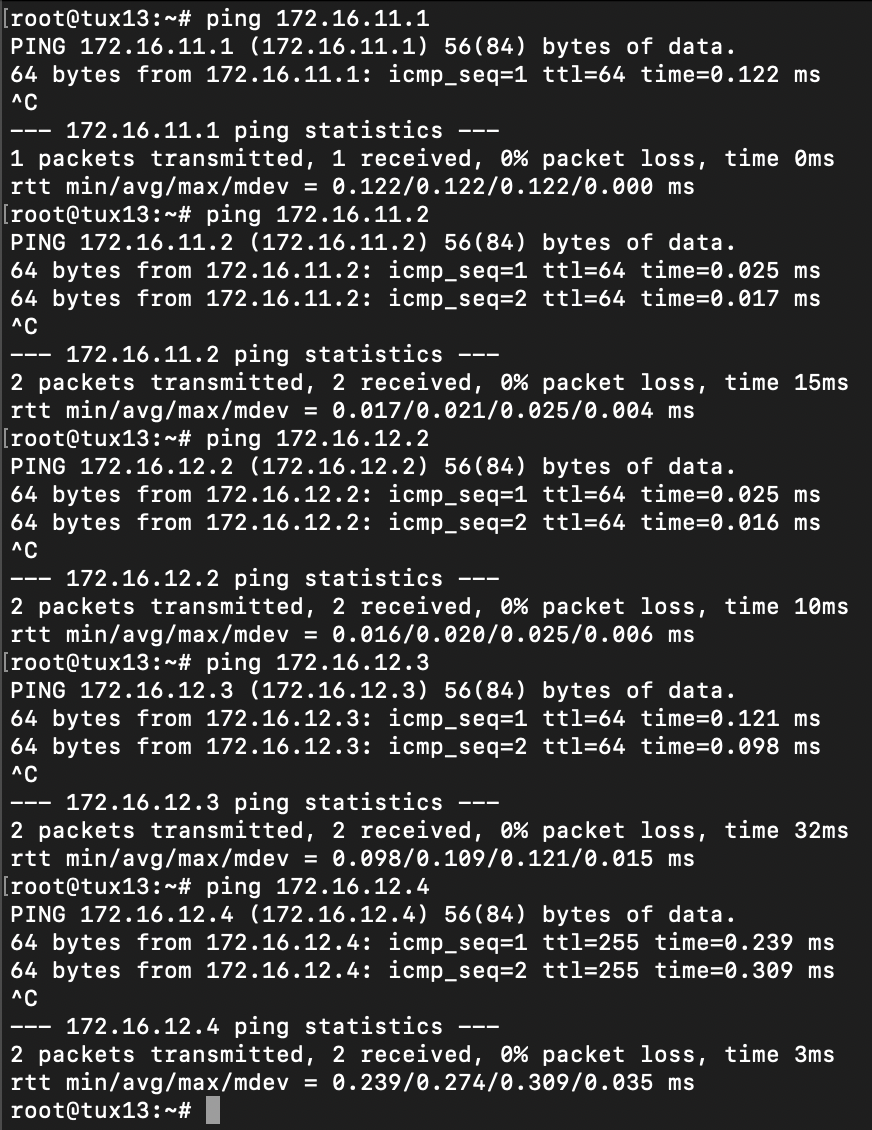
\includegraphics[width=.9\linewidth]{figs/int_routing/tux13_ping.png}
    \caption{Pings no Tux13}
    \label{fig:tux13_ping}
\end{figure}

\begin{figure}[H]
    \centering
    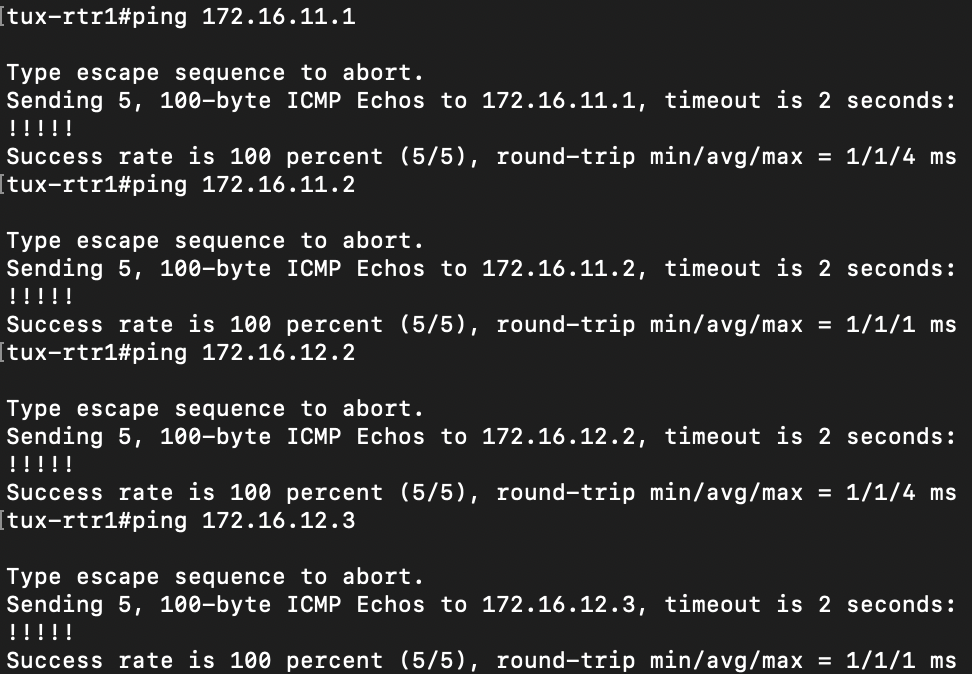
\includegraphics[width=.9\linewidth]{figs/int_routing/router_ping.png}
    \caption{Pings no Router de Bancada}
    \label{fig:router_ping}
\end{figure}

Através deste teste de conectividade provamos que todas as interfaces estão corretamente configuradas, assim como as respetivas \textit{Vlans}.

\pagebreak

\section{Teste de Routing do OSPF}

O acesso ao terminal do Router virtual criado nos \textit{Tuxs} é feito através do comando \verb|telnet localhost 2604|.
As \textit{Routing Tables} apresentadas pelos diferentes sistemas OSPF são as seguintes:

\begin{figure}[H]
    \centering
    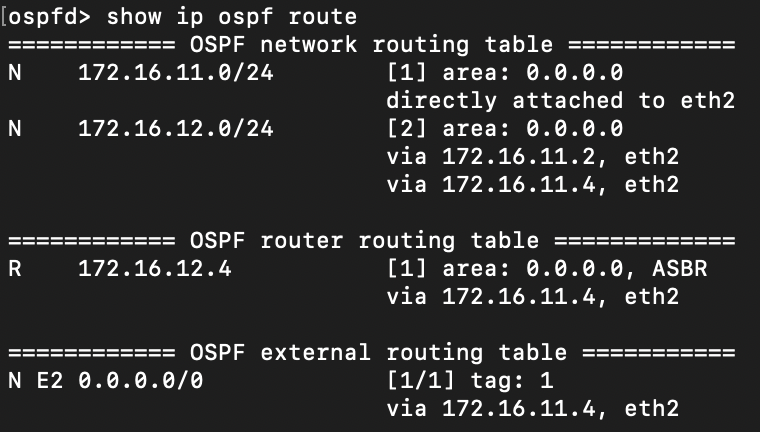
\includegraphics[width=.8\linewidth]{figs/int_routing/tux12_rt_1.png}
    \caption{Routing table no Tux12}
    \label{fig:tux12_rt_1}
\end{figure}

\begin{figure}[H]
    \centering
    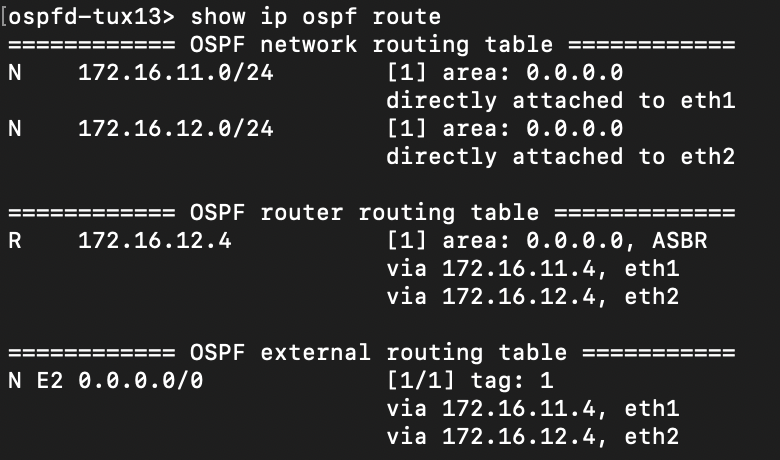
\includegraphics[width=.8\linewidth]{figs/int_routing/tux13_rt_1.png}
    \caption{Routing table no Tux13}
    \label{fig:tux13_rt_1}
\end{figure}

\begin{figure}[H]
    \centering
    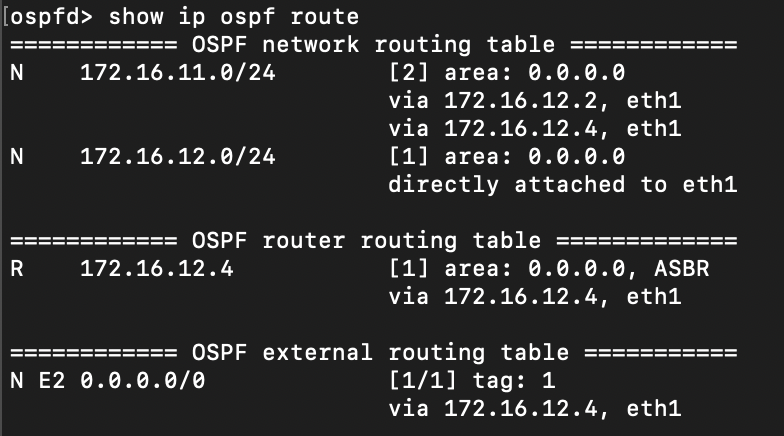
\includegraphics[width=.8\linewidth]{figs/int_routing/tux14_rt_1.png}
    \caption{Routing table no Tux14}
    \label{fig:tux14_rt_1}
\end{figure}

\begin{figure}[H]
    \centering
    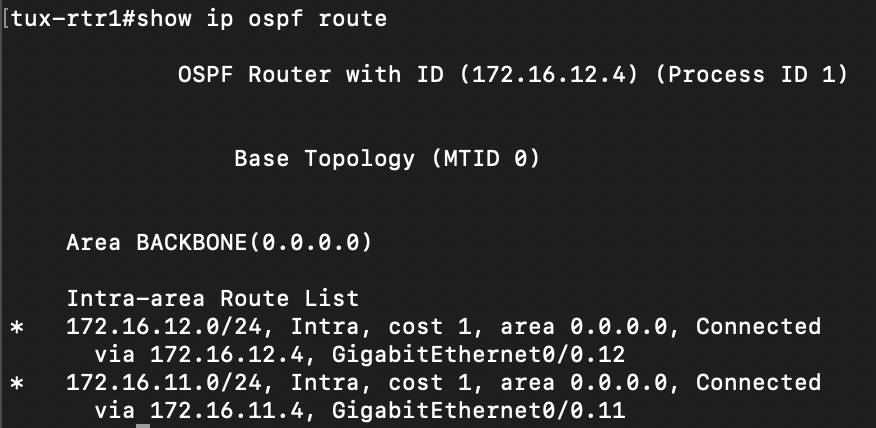
\includegraphics[width=.8\linewidth]{figs/int_routing/router_rt_1.png}
    \caption{Routing table no Router de Bancada}
    \label{fig:router_rt_1}
\end{figure}

Como se pode observar, todos os sistemas têm rotas para as duas \textit{networks}.

Se uma determinada interface fizer parte dessa \textit{Network} (mesma \textit{Vlan}), o custo associado a essa rota é de \textbf{1}.
Caso contrário, se tiver que passar por um outro Router para chegar à \textit{network}, o custo associado é de \textbf{2}.

O facto de estarem apresentadas como rotas possíveis para aceder a outra \textit{network}, quer o \textit{Tux13}, quer o Router de bancada, comprava que os custos associados a cada rota são iguais.
Isto cria uma malha de Router todos equilibrados e com a mesma \textit{bandwidth} aparente nas suas ligações.

Podemos também observar que o Router de Bancada (\verb|172.16.12.4|), é definido como o caminho \textit{default} em todos os \textit{Tuxs}.

\section{Teste com falha de ligação no OSPF}

Analisemos o cenário representado na figura \ref{fig:tux12_rt_1}.
A interface \textit{eth2} pertence à \textit{network} \verb|172.16.11.0/24|.
Deste modo, se este \textit{Tux} quiser comunicar com o IP \verb|172.16.12.2| que pertence a outra \textit{network}, precisa de passar por um router intermédio.

A tipologia de rede leva a uma preferência, como indicado na figura, de utilizar o \textit{Tux13}, pois corresponde a um menor numero de \textit{Hops} (1), do que passar pelo Router de bancada (2).
Um \verb|traceroute| comprova a teoria:

\begin{figure}[H]
    \centering
    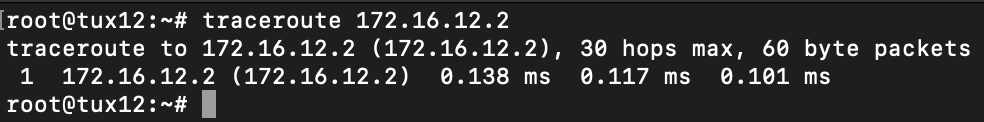
\includegraphics[width=.8\linewidth]{figs/int_routing/traceroute_1.png}
    \caption{Traceroute inicial}
    \label{fig:traceroute_1}
\end{figure}

No entanto, para testar a capacidade de multipath do protocolo OSPF, vamos simular um cenário de falha de uma ligação.
Neste caso, vamos desligar a interface eth1, que faz a ponte entre o \textit{Tux12 e Tux13} na \textit{network} \verb|172.16.11.0/24|.
Este era o caminho com menor custo para o cenário considerado.

Cortando esta ligação com o comando no \textit{Tux13} \verb|ifconfig eth1 down|, o único caminho possível é através do Router de bancada \verb|172.16.12.4|.
A tabela de \textit{routing} resultante no \textit{Tux12} para comunicação com a outra network já não apresenta o router no \textit{Tux13} como um caminho possível.

\begin{figure}[H]
    \centering
    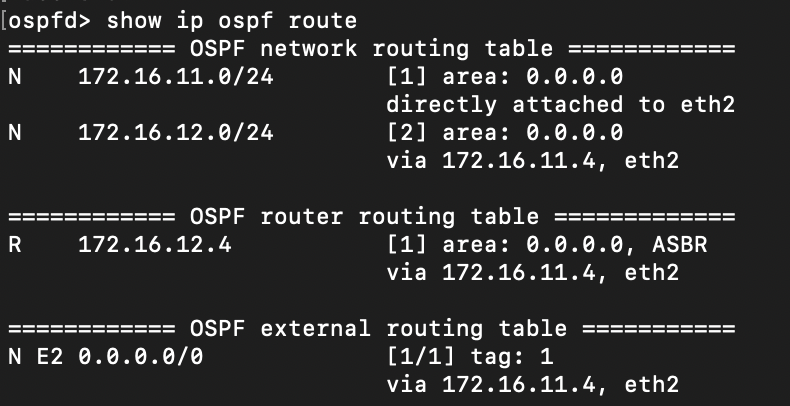
\includegraphics[width=.8\linewidth]{figs/int_routing/route_tb_2.png}
    \caption{Routing table no Tux12 depois da falha}
    \label{fig:route_tb_2}
\end{figure}


Um \verb|traceroute| confirma a rota apresentada pela tabela:

\begin{figure}[H]
    \centering
    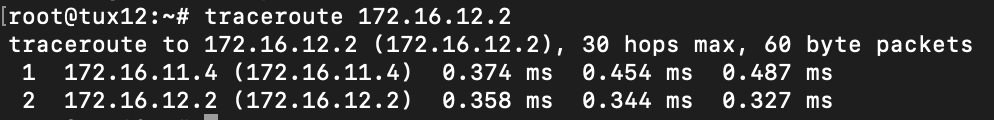
\includegraphics[width=.8\linewidth]{figs/int_routing/traceroute_2.png}
    \caption{Traceroute após modificação da rede}
    \label{fig:traceroute_2}
\end{figure}

É de notar que demora algum tempo até o sistema atualizar a informação sobre a modificação de uma ligação, neste caso que foi cortada.
No entanto, este tempo é curto, dado que por predefinição, o intervalo entre pacotes HELLO é de apenas 10 segundos
